\section{Liturgia światła}

\begin{itemize}
	\item Do poświęcenia ognia wychodzimy następująco:\\
	      \begin{center}
		      \begin{tabular}{rcl}
			                                   & \uparrow              & \smallskip                       \\
			                                   & \cc3~~~~\tt           & (z pustą kadzielnicą) \smallskip \\
			      (z tacką z granami i rylcem) & \aa2~~\ding{63}~~\aa1 & (z kropidłem)         \smallskip \\
			                                   & ministranci           & \smallskip                       \\
			                                   & \mm                   & (z paschałem)         \smallskip \\
			      (z mikrofonem)               & \cc2~~~~\cc1          & (z OHS)               \smallskip \\
			                                   & \ii~                  & (w kapie)             \smallskip \\
		      \end{tabular}
	      \end{center}
	\item \tt~ po dojściu do ogniska od razu wrzuca do środka węgielki, aby
	      się rozpaliły.
	\item stajemy przed kościołem w następujących pozycjach:
	      \begin{figure}[h]
		      \centering
		      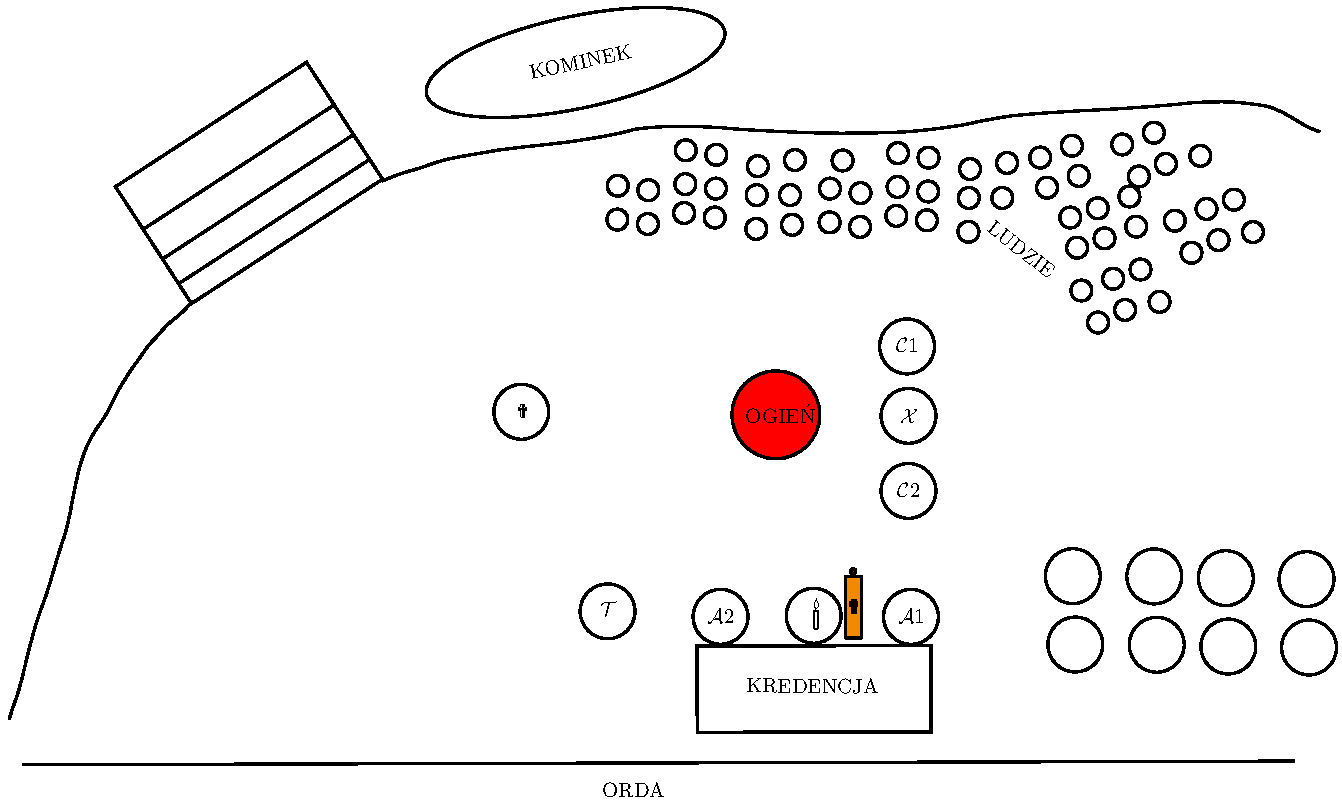
\includegraphics[width=0.8\linewidth]{Figures/Sobota/ogien.pdf}
		      \caption{Ustawienie na dworze}
		      \label{fig:ogien}
	      \end{figure}
	\item następuje poświęcenie ognia -- \ii~ odczytuje modlitwę z OHS
	\item po tym \tt~ wyciąga z ogniska węgielek, wkłada go to trybularza i
	      następuje zasypanie -- \cc2 trzyma kapę, aby się \textbf{nie
		      spaliła}
	\item pokropienie ogniska -- \aa1 podaje kropidło bezpośrednio \ii~ i
	      potem je odbiera. \cc2 przytrzymuje kapę, aby się \textbf{nie
		      spaliła}
	\item po pokropieniu ogniska następuje okadzenie ogniska. \cc2 przytrzymuje
	      kapę, aby się \textbf{nie spaliła}
	\item jeden z ministrantów odpala od ogniska świeczkę
	      ratunkową\footnote{najlepiej zamykany lampion} i idzie z
	      nią do kościoła
	\item następnie naprzeciwko \ii~ staje \mm~ z paschałem. Po jego lewej staje
	      \aa2 z tacką z rylcem. \ii~ kreśli wszystkie litery i cyfry.
	\item poświęcenie gran: trzykrotne pokropienie i okadzenie (\aa1 podaje i
	      odbiera kropidło, \tt~ podaje trybularz: bez zasypania!)
	\item \ii~ wkłada wszystkie grana w paschał.
	\item \cc1 odpala świeczkę od ognia i podaje \ii. Ten odpala paschał i potem
	      go błogosławi.
	\item \ii~ przebiera się w białą stułę i dalmatykę. Pomaga mu w tym \cc1
	      oraz \cc2.
	\item następuje zasypanie trybularza
	\item kantorzy podejmują śpiew \textit{Inventor rutili}
	\item procesja z paschałem wchodzi do kościoła:
	      \begin{center}
		      \uparrow \smallskip\\
		      \cc3~~~\tt \smallskip\\
		      \aa2~~\ding{63}~~\aa1 \smallskip\\
		      \ii \smallskip\\
		      \cc2~~~\cc1 \smallskip\\
		      \mm \smallskip\\
		      ministranci
	      \end{center}
	\item trzykrotne Lumen Christi:  (patrz Rys.\ref{fig:procesja})
	      \begin{itemize}
		      \item przy kracie wejściowej od wejścia zachodniego (świece
		            zapalają ministranci)
		      \item w połowie nawy głównej, na wysokości ołtarza NOM (świece
		            zapalają wierni)
		      \item w prezbiterium
	      \end{itemize}
	\item przed trzecim \textit{Lumen Christi} \ding{63} z \aa\aa~ idą od razu do
	      prezbiterium i ustawia się na swoich miejscach (naprzeciwko
	      Paschału / obok kredencji) (patrz Rys.\ref{fig:exultet})
	\item po trzecim \textit{Lumen Christi} \mm~ odbiera paschał od \ii~ i wraz
	      z \cc2 idą umieścić go na stojaku
\end{itemize}

\begin{figure}[h]
	\centering
	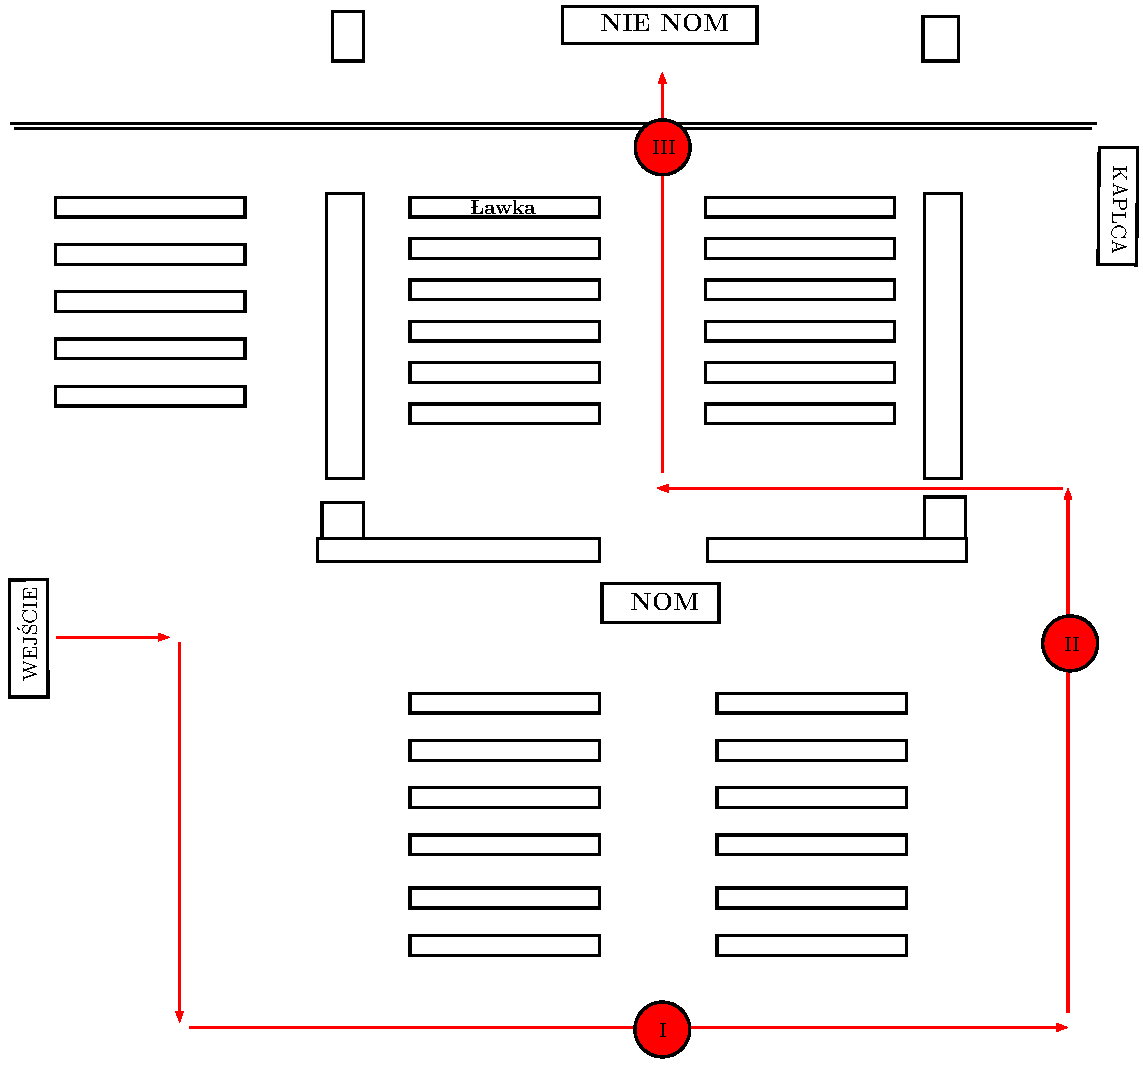
\includegraphics[width=0.6\linewidth]{Figures/Sobota/procesja.pdf}
	\caption{Prosceja z Pachałem -- czerwone kropki oznaczają miejsca,
		w których kapłan śpiewa \textit{Lumen Christi}}
	\label{fig:procesja}
\end{figure}

